\uuid{sx3x}
\exo7id{5817}
\titre{exo7 5817}
\auteur{rouget}
\organisation{exo7}
\datecreate{2010-10-16}
\isIndication{false}
\isCorrection{true}
\chapitre{Conique}
\sousChapitre{Conique}
\module{Géométrie}
\niveau{L2}
\difficulte{}

\contenu{
\texte{

}
\begin{enumerate}
    \item \question{Montrer que toute courbe de degré inférieur ou égal à $2$ admet une représentation paramétrique de la forme

\begin{center}
$\left\{
\begin{array}{l}
x(t)=\frac{P(t)}{R(t)}\\
y(t)=\frac{Q(t)}{R(t)}
\end{array}
\right.$
\end{center}

où $P$, $Q$ et $R$ sont des polynômes de degré inférieur ou égal à $2$ et montrer réciproquement que toute courbe paramétrée du type précédent est une courbe de degré inférieur ou égal à $2$.}
\reponse{Une ellipse (privée d'un point) admet une représentation paramétrique de la forme $\left\{
\begin{array}{l}
a\frac{1-t^2}{1+t^2}\\
\rule{0mm}{6mm}b\frac{2t}{1+t^2}
\end{array}
\right.$, $t\in\Rr$, dans un repère adapté. Une branche d'hyperbole admet une représentation paramétrique de la forme 
 $\left\{
\begin{array}{l}
a\frac{1+t^2}{1-t^2}\\
b\frac{2t}{1-t^2}
\end{array}
\right.$, $t\in]-1,1[$, dans un repère adapté. Une parabole admet une représentation paramétrique de la forme 
 $\left\{
\begin{array}{l}
\frac{t^2}{2p}\\
\rule{0mm}{6mm}t
\end{array}
\right.$, dans un repère adapté ...

Réciproquement, si la courbe admet une paramétrisation du type de l'énoncé, les six polynômes $P^2$, $PQ$, $Q^2$, $PR$, $QR$ et $R^2$ sont dans $\Rr_4[X]$ qui est de dimension $5$ et donc sont linéairement dépendants. On en déduit qu'il existe $(a,b,c,d,e,f)\neq(0,0,0,0,0,0)$ tel que 
$aP^2+2bPQ+cQ^2+2dPR+2eQR+fR^2 = 0$ ou encore tel que pour tout réel $t$ tel que $R(t)\neq 0$,

\begin{center}
$a\left(\frac{P(t)}{R(t)}\right)^2 +2b\frac{P(t)}{R(t)}\times\frac{Q(t)}{R(t)}+c\left(\frac{Q(t)}{R(t)}\right)^2+2d\frac{P(t)}{R(t)}+2e\frac{Q(t)}{R(t)}+f = 0$.
\end{center}

Le support de l'arc est donc contenu dans la courbe d'équation $ax^2 + 2bxy + cy^2 + 2dx + 2ey + f = 0$ où $(a,b,c,d,e,f)\neq(0,0,0,0,0,0))$.}
    \item \question{Etudier la courbe $\left\{
\begin{array}{l}
x=\frac{2t+1}{t^2+2t-1}\\
y=\frac{t^2-1}{t^2+2t-1}
\end{array}
\right.$.}
\reponse{Construction de la courbe $\left\{
\begin{array}{l}
x=\frac{2t+1}{t^2+2t-1}\\
y=\frac{t^2-1}{t^2+2t-1}
\end{array}
\right.$.

$$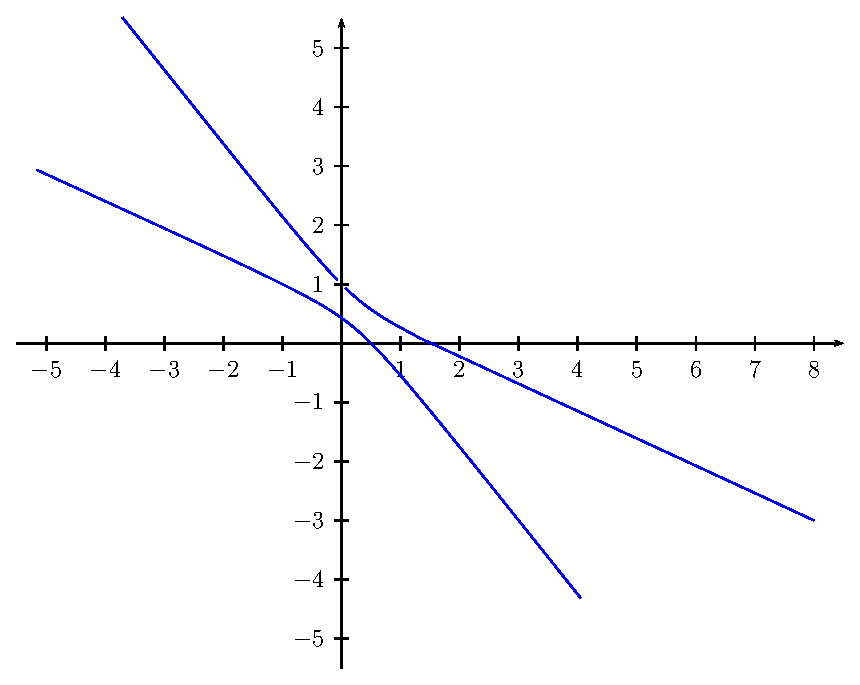
\includegraphics{../images/img005817-1}$$}
\end{enumerate}
}
